\documentclass[journal,12pt,twocolumn]{IEEEtran}

\usepackage{setspace}
\usepackage{gensymb}
\singlespacing
\usepackage[cmex10]{amsmath}

\usepackage{amsthm}

\usepackage{mathrsfs}
\usepackage{txfonts}
\usepackage{stfloats}
\usepackage{bm}
\usepackage{cite}
\usepackage{cases}
\usepackage{subfig}

\usepackage{longtable}
\usepackage{multirow}

\usepackage{enumitem}
\usepackage{mathtools}
\usepackage{steinmetz}
\usepackage{tikz}
\usepackage{circuitikz}
\usepackage{verbatim}
\usepackage{tfrupee}
\usepackage[breaklinks=true]{hyperref}
\usepackage{graphicx}
\usepackage{tkz-euclide}

\usetikzlibrary{calc,math}
\usepackage{listings}
    \usepackage{color}                                            %%
    \usepackage{array}                                            %%
    \usepackage{longtable}                                        %%
    \usepackage{calc}                                             %%
    \usepackage{multirow}                                         %%
    \usepackage{hhline}                                           %%
    \usepackage{ifthen}                                           %%
    \usepackage{lscape}     
\usepackage{multicol}
\usepackage{chngcntr}

\usetikzlibrary{matrix,positioning}
\DeclareMathOperator*{\Res}{Res}

\renewcommand\thesection{\arabic{section}}
\renewcommand\thesubsection{\thesection.\arabic{subsection}}
\renewcommand\thesubsubsection{\thesubsection.\arabic{subsubsection}}

\renewcommand\thesectiondis{\arabic{section}}
\renewcommand\thesubsectiondis{\thesectiondis.\arabic{subsection}}
\renewcommand\thesubsubsectiondis{\thesubsectiondis.\arabic{subsubsection}}


\hyphenation{op-tical net-works semi-conduc-tor}
\def\inputGnumericTable{}                                 %%

\lstset{
%language=C,
frame=single, 
breaklines=true,
columns=fullflexible
}
\begin{document}


\newtheorem{theorem}{Theorem}[section]
\newtheorem{problem}{Problem}
\newtheorem{proposition}{Proposition}[section]
\newtheorem{lemma}{Lemma}[section]
\newtheorem{corollary}[theorem]{Corollary}
\newtheorem{example}{Example}[section]
\newtheorem{definition}[problem]{Definition}

\newcommand{\BEQA}{\begin{eqnarray}}
\newcommand{\EEQA}{\end{eqnarray}}
\newcommand{\define}{\stackrel{\triangle}{=}}
\bibliographystyle{IEEEtran}
\raggedbottom
\setlength{\parindent}{0pt}
\providecommand{\mbf}{\mathbf}
\providecommand{\pr}[1]{\ensuremath{\Pr\left(#1\right)}}
\providecommand{\qfunc}[1]{\ensuremath{Q\left(#1\right)}}
\providecommand{\sbrak}[1]{\ensuremath{{}\left[#1\right]}}
\providecommand{\lsbrak}[1]{\ensuremath{{}\left[#1\right.}}
\providecommand{\rsbrak}[1]{\ensuremath{{}\left.#1\right]}}
\providecommand{\brak}[1]{\ensuremath{\left(#1\right)}}
\providecommand{\lbrak}[1]{\ensuremath{\left(#1\right.}}
\providecommand{\rbrak}[1]{\ensuremath{\left.#1\right)}}
\providecommand{\cbrak}[1]{\ensuremath{\left\{#1\right\}}}
\providecommand{\lcbrak}[1]{\ensuremath{\left\{#1\right.}}
\providecommand{\rcbrak}[1]{\ensuremath{\left.#1\right\}}}
\theoremstyle{remark}
\newtheorem{rem}{Remark}
\newcommand{\sgn}{\mathop{\mathrm{sgn}}}
% \providecommand{\abs}[1]{\left\vert#1\right\vert}
% \providecommand{\res}[1]{\Res\displaylimits_{#1}} 
% \providecommand{\norm}[1]{\left\lVert#1\right\rVert}
% %\providecommand{\norm}[1]{\lVert#1\rVert}
% \providecommand{\mtx}[1]{\mathbf{#1}}
% \providecommand{\mean}[1]{E\left[ #1 \right]}
\providecommand{\fourier}{\overset{\mathcal{F}}{ \rightleftharpoons}}
%\providecommand{\hilbert}{\overset{\mathcal{H}}{ \rightleftharpoons}}
\providecommand{\system}{\overset{\mathcal{H}}{ \longleftrightarrow}}
	%\newcommand{\solution}[2]{\textbf{Solution:}{#1}}
\newcommand{\solution}{\noindent \textbf{Solution: }}
\newcommand{\cosec}{\,\text{cosec}\,}
\providecommand{\dec}[2]{\ensuremath{\overset{#1}{\underset{#2}{\gtrless}}}}
\newcommand{\myvec}[1]{\ensuremath{\begin{pmatrix}#1\end{pmatrix}}}
\newcommand{\mydet}[1]{\ensuremath{\begin{vmatrix}#1\end{vmatrix}}}
\numberwithin{equation}{subsection}
\makeatletter
\@addtoreset{figure}{problem}
\makeatother
\let\StandardTheFigure\thefigure
\let\vec\mathbf
\renewcommand{\thefigure}{\theproblem}
\def\putbox#1#2#3{\makebox[0in][l]{\makebox[#1][l]{}\raisebox{\baselineskip}[0in][0in]{\raisebox{#2}[0in][0in]{#3}}}}
     \def\rightbox#1{\makebox[0in][r]{#1}}
     \def\centbox#1{\makebox[0in]{#1}}
     \def\topbox#1{\raisebox{-\baselineskip}[0in][0in]{#1}}
     \def\midbox#1{\raisebox{-0.5\baselineskip}[0in][0in]{#1}}
\vspace{3cm}
\title{Assignment 1}
\author{Pragna Mamidipaka - EE20BTECH11026}
\maketitle
\newpage
\bigskip
\renewcommand{\thefigure}{\theenumi}
\renewcommand{\thetable}{\theenumi}
Download all latex-tikz codes from 
%
\begin{lstlisting}
https://github.com/Pymamid/C-and-Data-Structures/blob/main/Assignment1/Assignment1.tex
\end{lstlisting}
\section{Problem}
(Q 29) Consider the following C function.
\begin{lstlisting}
#include<stdio.h>
void fun1(char *s1, char *s2){
    char *tmp;
    tmp = s1;
    s1 = s2;
    s2 = tmp;
}
void fun2(char **s1, char **s2){
    char *tmp;
    tmp = *s1;
    *s1 = *s2;
    *s2 = tmp;
}
int main(){
    char *str1 = "Hi", *str2 = "Bye";
    fun1(str1, str2); 
    printf("%s %s ", str1, str2);
    fun2(&str1, &str2); 
    printf("%s %s", str1, str2);
    return 0;
}
\end{lstlisting}
The output of the program above is

\begin{enumerate}
    \item Hi Bye Bye Hi
    \item Hi Bye Hi Bye
    \item Bye Hi Hi Bye
    \item Bye Hi Bye Hi
\end{enumerate}
\section{Solution}
Answer : The output of the above program is:
\newline
1) Hi Bye Bye Hi
\bigbreak
\textbf{Explanation}
\newline
\newline
\textit{Str1} and \textit{Str2} before call to \textit{fun1}:
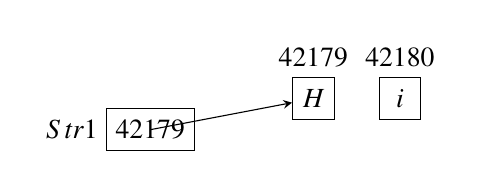
\begin{tikzpicture}[pmat/.style={matrix of math nodes,nodes in empty cells,
    nodes={minimum size=1.5em,anchor=center},
    column sep=-\pgflinewidth,row sep=-\pgflinewidth}]
 \node[pmat,column 2/.style={nodes={draw}}] (STU)
  {Str1 & 42179\\};
 \node[above right=0.0em and 2em of STU.east,pmat,row 2/.style={nodes={draw}}] (TU)
  {42179 & 42180\\ H & i \\};
 \path[stealth-]  foreach \X in {1} {(TU-2-1) edge (STU-\X-2.center)};
\end{tikzpicture}
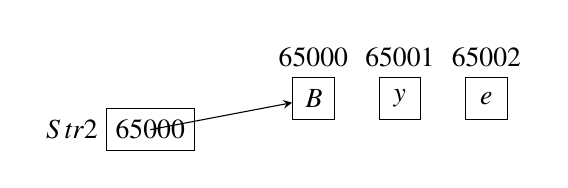
\begin{tikzpicture}[pmat/.style={matrix of math nodes,nodes in empty cells,
    nodes={minimum size=1.5em,anchor=center},
    column sep=-\pgflinewidth,row sep=-\pgflinewidth}]
 \node[pmat,column 2/.style={nodes={draw}}] (STU)
  {Str2 & 65000\\};
 \node[above right=0.0em and 2em of STU.east,pmat,row 2/.style={nodes={draw}}] (TU)
  {65000 & 65001 & 65002\\ B & y & e \\};
 \path[stealth-]  foreach \X in {1} {(TU-2-1) edge (STU-\X-2.center)};
\end{tikzpicture}
\newline
\newline\newline
The function \textit{fun1} is call-by-value. In this mechanism, the \underline{values} of actual parameters get copied to formal parameters and the modifications performed on formal parameters will not be updated on actual parameters.
Therefore, \textit{str1} and \textit{str2} still point to their old values. \textit{s1} and \textit{s2} point to Bye and Hi respectively.
\newline\newline
i.e., after call to \textit{fun1}, \newline
str1 points to \textbf{Hi} \newline
str2 points to \textbf{Bye}
\newline
\newline
The values of Str1 and Str2 get passed to S1 and S2:

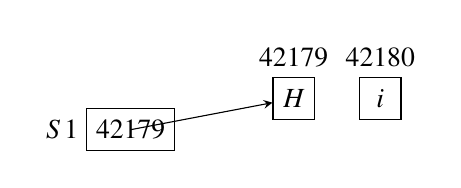
\begin{tikzpicture}[pmat/.style={matrix of math nodes,nodes in empty cells,
    nodes={minimum size=1.5em,anchor=center},
    column sep=-\pgflinewidth,row sep=-\pgflinewidth}]
 \node[pmat,column 2/.style={nodes={draw}}] (STU)
  {S1 & 42179\\};
 \node[above right=0.0em and 2em of STU.east,pmat,row 2/.style={nodes={draw}}] (TU)
  {42179 & 42180\\ H & i \\};
 \path[stealth-]  foreach \X in {1} {(TU-2-1) edge (STU-\X-2.center)};
\end{tikzpicture}
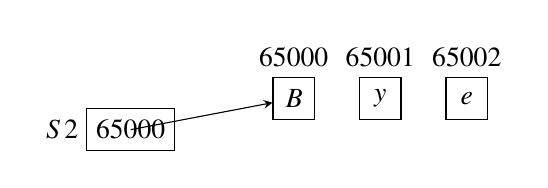
\begin{tikzpicture}[pmat/.style={matrix of math nodes,nodes in empty cells,
    nodes={minimum size=1.5em,anchor=center},
    column sep=-\pgflinewidth,row sep=-\pgflinewidth}]
 \node[pmat,column 2/.style={nodes={draw}}] (STU)
  {S2 & 65000\\};
 \node[above right=0.0em and 2em of STU.east,pmat,row 2/.style={nodes={draw}}] (TU)
  {65000 & 65001 & 65002\\ B & y & e \\};
 \path[stealth-]  foreach \X in {1} {(TU-2-1) edge (STU-\X-2.center)};
\end{tikzpicture}
\newline\newline
After execution of \textit{fun1}, the values of S1 and S2 get swapped, but Str1 and Str2 remain unchanged.
\newline
\newline
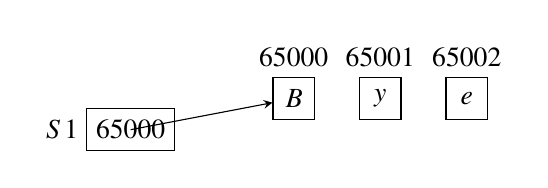
\begin{tikzpicture}[pmat/.style={matrix of math nodes,nodes in empty cells,
    nodes={minimum size=1.5em,anchor=center},
    column sep=-\pgflinewidth,row sep=-\pgflinewidth}]
 \node[pmat,column 2/.style={nodes={draw}}] (STU)
  {S1 & 65000\\};
 \node[above right=0.0em and 2em of STU.east,pmat,row 2/.style={nodes={draw}}] (TU)
  {65000 & 65001 & 65002\\ B & y & e \\};
 \path[stealth-]  foreach \X in {1} {(TU-2-1) edge (STU-\X-2.center)};
\end{tikzpicture}
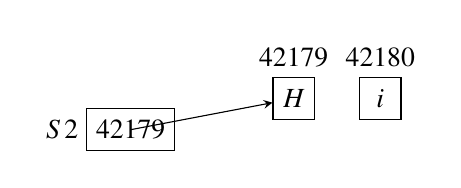
\begin{tikzpicture}[pmat/.style={matrix of math nodes,nodes in empty cells,
    nodes={minimum size=1.5em,anchor=center},
    column sep=-\pgflinewidth,row sep=-\pgflinewidth}]
 \node[pmat,column 2/.style={nodes={draw}}] (STU)
  {S2 & 42179\\};
 \node[above right=0.0em and 2em of STU.east,pmat,row 2/.style={nodes={draw}}] (TU)
  {42179 & 42180\\ H & i \\};
 \path[stealth-]  foreach \X in {1} {(TU-2-1) edge (STU-\X-2.center)};
\end{tikzpicture}

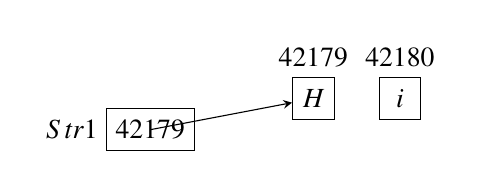
\begin{tikzpicture}[pmat/.style={matrix of math nodes,nodes in empty cells,
    nodes={minimum size=1.5em,anchor=center},
    column sep=-\pgflinewidth,row sep=-\pgflinewidth}]
 \node[pmat,column 2/.style={nodes={draw}}] (STU)
  {Str1 & 42179\\};
 \node[above right=0.0em and 2em of STU.east,pmat,row 2/.style={nodes={draw}}] (TU)
  {42179 & 42180\\ H & i \\};
 \path[stealth-]  foreach \X in {1} {(TU-2-1) edge (STU-\X-2.center)};
\end{tikzpicture}
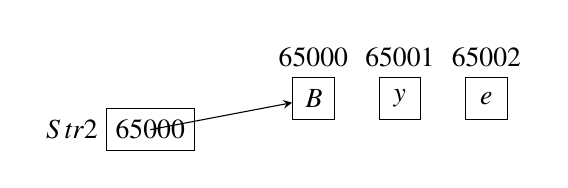
\begin{tikzpicture}[pmat/.style={matrix of math nodes,nodes in empty cells,
    nodes={minimum size=1.5em,anchor=center},
    column sep=-\pgflinewidth,row sep=-\pgflinewidth}]
 \node[pmat,column 2/.style={nodes={draw}}] (STU)
  {Str2 & 65000\\};
 \node[above right=0.0em and 2em of STU.east,pmat,row 2/.style={nodes={draw}}] (TU)
  {65000 & 65001 & 65002\\ B & y & e \\};
 \path[stealth-]  foreach \X in {1} {(TU-2-1) edge (STU-\X-2.center)};
\end{tikzpicture}
\newline
\newline
\newline
\newline

The function \textit{fun2} is call-by-reference. In this mechanism, the \underline{address} of actual parameters get copied to formal parameters. Therefore, the modifications performed via formal parameters will be updated on actual parameters.
Therefore, the values in \textit{str1} and \textit{str2} get interchanged by calling the second function.
\newline\newline
i.e., after call to \textit{fun2}, \newline
str1 points to \textbf{Bye} \newline
str2 points to \textbf{Hi}
\newline
\newline
Address of str1 and str2 are passed to \textit{fun2}:
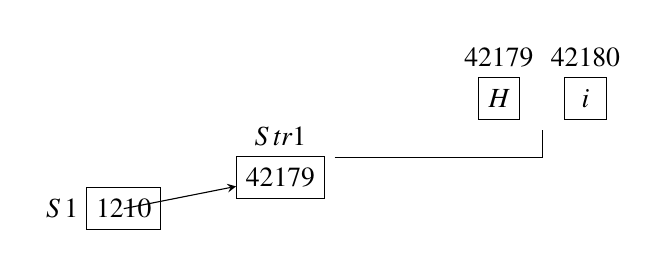
\begin{tikzpicture}[pmat/.style={matrix of math nodes,nodes in empty cells,
    nodes={minimum size=1.5em,anchor=center},
    column sep=-\pgflinewidth,row sep=-\pgflinewidth}]
 \node[pmat,column 2/.style={nodes={draw}}] (STU)
  {S1 & 1210\\};
 \node[above right=0.0em and 2em of STU.east,pmat,row 2/.style={nodes={draw}}] (TUS)
  {Str1 \\ 42179  \\};
 \path[stealth-]  foreach \X in {1} {(TUS-2-1) edge (STU-\X-2.center)};
 \node[above right=1em and 4em of TUS.east,pmat,row 2/.style={nodes={draw}}] (TU)
  {42179 & 42180\\ H & i \\};
  \draw[-, to path={-| (\tikztotarget)}]
  (TUS) edge (TU) ;

\end{tikzpicture}
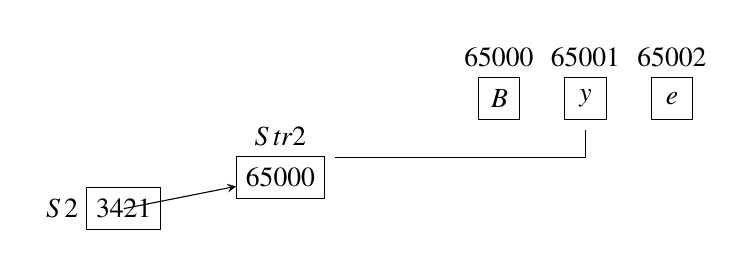
\begin{tikzpicture}[pmat/.style={matrix of math nodes,nodes in empty cells,
    nodes={minimum size=1.5em,anchor=center},
    column sep=-\pgflinewidth,row sep=-\pgflinewidth}]
 \node[pmat,column 2/.style={nodes={draw}}] (STU)
  {S2 & 3421\\};
 \node[above right=0.0em and 2em of STU.east,pmat,row 2/.style={nodes={draw}}] (TUS)
  {Str2 \\ 65000  \\};
 \path[stealth-]  foreach \X in {1} {(TUS-2-1) edge (STU-\X-2.center)};
 \node[above right=1em and 4em of TUS.east,pmat,row 2/.style={nodes={draw}}] (TU)
  {65000 & 65001 & 65002\\ B & y & e\\};
  \draw[-, to path={-| (\tikztotarget)}]
  (TUS) edge (TU) ;

\end{tikzpicture}
\newline
\newline
\bigbreak
\textit{fun2} swaps the values dereferenced by S1 and S2:
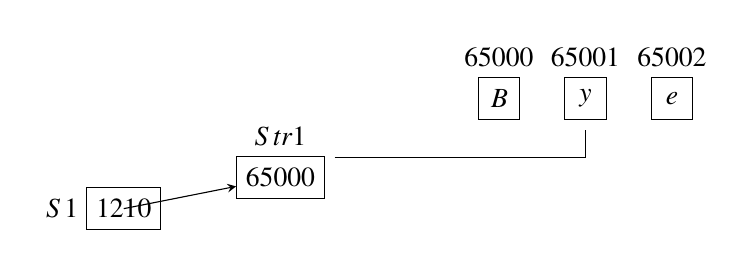
\begin{tikzpicture}[pmat/.style={matrix of math nodes,nodes in empty cells,
    nodes={minimum size=1.5em,anchor=center},
    column sep=-\pgflinewidth,row sep=-\pgflinewidth}]
 \node[pmat,column 2/.style={nodes={draw}}] (STU)
  {S1 & 1210\\};
 \node[above right=0.0em and 2em of STU.east,pmat,row 2/.style={nodes={draw}}] (TUS)
  {Str1 \\ 65000  \\};
 \path[stealth-]  foreach \X in {1} {(TUS-2-1) edge (STU-\X-2.center)};
 \node[above right=1em and 4em of TUS.east,pmat,row 2/.style={nodes={draw}}] (TU)
  {65000 & 65001 & 65002\\ B & y & e\\};
  \draw[-, to path={-| (\tikztotarget)}]
  (TUS) edge (TU) ;

\end{tikzpicture}
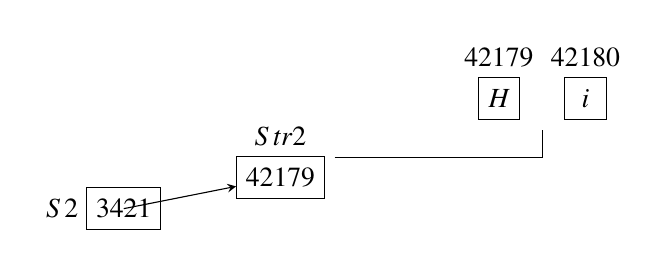
\begin{tikzpicture}[pmat/.style={matrix of math nodes,nodes in empty cells,
    nodes={minimum size=1.5em,anchor=center},
    column sep=-\pgflinewidth,row sep=-\pgflinewidth}]
 \node[pmat,column 2/.style={nodes={draw}}] (STU)
  {S2 & 3421\\};
 \node[above right=0.0em and 2em of STU.east,pmat,row 2/.style={nodes={draw}}] (TUS)
  {Str2 \\ 42179  \\};
 \path[stealth-]  foreach \X in {1} {(TUS-2-1) edge (STU-\X-2.center)};
 \node[above right=1em and 4em of TUS.east,pmat,row 2/.style={nodes={draw}}] (TU)
  {42179 & 42180\\ H & i \\};
  \draw[-, to path={-| (\tikztotarget)}]
  (TUS) edge (TU) ;

\end{tikzpicture}

\end{document}